%% Adaptado de 
%% http://www.ctan.org/tex-archive/macros/latex/contrib/IEEEtran/
%% Traduzido para o congresso de IC da USP
%%*****************************************************************************
% Não modificar

\documentclass[twoside,conference,a4paper]{IEEEtran}
\makeatletter
\def\endthebibliography{%
  \def\@noitemerr{\@latex@warning{Empty `thebibliography' environment}}%
  \endlist
}
\makeatother

%******************************************************************************
% Não modificar
\usepackage{IEEEtsup} % Definições complementares e modificações.
\usepackage[utf8x]{inputenc} % Disponibiliza acentos.
\usepackage[english,brazil]{babel}
%% Disponibiliza Inglês e Português do Brasil.
\usepackage{latexsym,amsfonts,amssymb} % Disponibiliza fontes adicionais.
\usepackage{theorem} 
\usepackage[cmex10]{amsmath} % Pacote matemático básico 
\usepackage{url} 
%\usepackage[portuges,brazil,english]{babel}
\usepackage{graphicx}
\usepackage{amsmath}
\usepackage{amssymb}
\usepackage{color}
\usepackage[pagebackref=true,breaklinks=true,letterpaper=true,colorlinks,bookmarks=false]{hyperref}
\usepackage[tight,footnotesize]{subfigure} 
\usepackage[noadjust]{cite} % Disponibiliza melhorias em citações.
\usepackage[]{algorithm2e}
\DeclareMathOperator*{\argmin}{\arg\!\min}

%%*****************************************************************************

\begin{document}
    \selectlanguage{english}
    \renewcommand{\IEEEkeywordsname}{Keywords}
    
    %%*****************************************************************************
    
    \urlstyle{tt}
    % Indicar o nome do autor e o curso/nível (grad-mestrado-doutorado-especial)
    \title{Estudo Dirigido - Teoria dos Jogos Algorítmica}
    \author{%
        \IEEEauthorblockN{Luiz Eduardo Cartolano\,\IEEEauthorrefmark{1},
                          Rafael C. S. Schouery\, \IEEEauthorrefmark{1}}
        \IEEEauthorblockA{\IEEEauthorrefmark{1}%
                           Instituto de Computação, Universidade Estadual de Campinas - UNICAMP, Campinas-SP, Brasil}
    }
    
    %%*****************************************************************************
    
    \maketitle
    
    %%*****************************************************************************
    % Resumo do trabalho
    % \begin{abstract}
        
    % \end{abstract}

    
    % Indique três palavras-chave que descrevem o trabalho
    \begin{IEEEkeywords}
        
    \end{IEEEkeywords}
    
    %%*****************************************************************************
    % Modifique as seções de acordo com o seu projeto
    \section{Introdução}
        A Teoria dos Jogos Algorítmica é uma área na interseção entre teoria dos jogos e ciência da computação, com o objetivo de entender e projetar algoritmos em ambientes estratégicos. Ela visa modelar situações nas quais múltiplas partes interagem ou afetam seus resultados entre si.
        
        O objetivo do relatório em questão é apresentar os conteúdos estudados durante o semestre na disciplina de Estudo Dirigido (MC032) do Instituto de Computação da Unicamp.
        
        Para guiar o estudo serão usados livros e artigos da área. Que serão informados aqui com o passar do tempo. Para dar início aos estudos usaremos o livro \cite{algorithmic-game-theory-book}, a fim de introduzir o aluno aos conceitos iniciais e também mais avançados da área.
        
    
    \section{Conceitos Iniciais sobre Teoria dos Jogos}
        A fim de explicar os conceitos iniciais estudados, buscaremos associar e exemplificar as definições usando situações de jogos clássicos apresentados, como o \emph{Dilema do Prisioneiro}, \emph{Jogo da Poluição}, \emph{Jogo do Roteamento}, entre outros.
        
        \subsection{Jogo}
            No \emph{Dilema do Prisioneiro}, dois prisioneiros estão em julgamento por um crime. Cada jogador tem a possibilidade de confessar ou não o crime.
            
            Se analisarmos atentamente a descrição do \emph{Dilema do Prisioneiro}, encontramos todas as características necessárias para caracterizar um jogo. Temos um conjunto de dois jogadores (prisioneiros um e dois) e também possuímos um conjunto de estratégias possíveis para cada jogador (confessar ou permanecer em silêncio). 
            
            Ou seja, de maneira informal, podemos dizer que um jogo é caracterizado por um conjunto de jogadores, no qual cada jogador tem um conjunto de possíveis ações (estratégias) que podem ser tomadas, com diferentes probabilidades.
            
            De maneira mais formal, a definição de um jogo pode ser feita da seguinte maneira:\\ \\
            \textbf{Definição 2.1.} Definimos como jogo a família de três conjuntos: um conjunto de n jogadores $P = {1, 2, ..., n};$ uma família de $n$ conjuntos de estratégias possíveis $S = {S_1, S_2, ..., S_n}$, na qual $S_i$ é o conjunto de estratégias possíveis do jogador $i$, para todo $i \in P$; e um conjunto de funções $U = {u_1, u_2, ..., u_n}$, no qual $u_i$ é uma função $S \xrightarrow{} R$ que define a utilidade do jogador i de acordo com todas as estratégias escolhidas, em que $S = S_1 × S_2... × S_n$.
        
        \subsection{Como Representar um Jogo}
            Cada possível estratégia tomada por um jogador costuma ter sequências no jogo, voltemos ao \emph{Dilema do Prisioneiro}. Se ambos os jogadores permanecerem em silêncio, cumprem uma pena curta, de dois anos. Caso apenas um deles confesse, o que confessou cumpre uma pena de apenas um ano, enquanto o outro passa os próximos cinco anos preso. Por fim, se ambos confessarem, cumprem juntos quatro anos de prisão. Essa situação pode ser vista na Matriz \ref{table1: matriz-custo}.
            
            O \emph{Dilema do Prisioneiro} pode ser representado como foi feito na Matriz \ref{table1: matriz-custo}, a essa forma dá-se o nome de \emph{forma explícita}. Esta, é uma maneira super útil e eficiente para representar os jogos, especialmente em situações nas quais existem dois jogadores.
            
            A \emph{forma explícita} contudo, costuma ser bem restritiva e pouco utilizável quando tratamos de jogos com mais de dois jogadores, ou quando cada jogador possui muitas estratégias possíveis de adotar. 
            
            Seguindo a lógica do \emph{Dilema do Prisioneiro}, imaginem que, ao invés de dois prisioneiros no julgamento, existisse um número arbitrário $n$ deles, cada um com duas estratégias possíveis. Nessa situação, haveriam $2^n$ vetores de estratégias possíveis, e a \emph{forma explícita} de representação torna-se inimaginável. Além de extremamente ineficiente, é claro.
            
            Outra situação na qual a \emph{forma explícita} deixa de ser uma opção pode ser vista em jogos como os de roteamento. Imagine uma situação que descreva $n$ jogadores compartilhando uma mesma banda de internet. E a ação tomada por cada jogador é escolher a quantidade de banda (em porcentagem) que ele irá utilizar. Ou seja, qualquer valor $x \in [0,1]$ é uma estratégia possível, logo, temos um conjunto infinito de estratégias.
        
        \subsection{Estratégia Dominante}
            Para esta seção iremos, novamente, analisar a Matriz \ref{table1: matriz-custo}, dessa vez, visando entender qual seria a melhor estratégia para o prisioneiro $P_i$. Analisando o tempo de prisão ao qual cada jogador seria submetido, a melhor estratégia, para ambos seria permanecer em silêncio. Contudo, essa é uma situação que chamamos de instável, pois, a qualquer momento, o outro prisioneiro poderia resolver diminuir o seu tempo de prisão tomando a atitude de confessar. Portanto, podemos concluir que, a melhor estratégia que pode ser tomada \textbf{individualmente} é a de confessar. Além de estável, afinal é impossível que qualquer um dos jogadores diminua o tempo de prisão nesse caso, essa é uma \textbf{estratégia dominante}, isto é, a \emph{única} melhor estratégia que pode ser tomada de maneira individual.
            
            De maneira mais formal, a definição de uma estratégia dominante pode ser feita da seguinte maneira:\\ \\
            \textbf{Definição 2.2.} Um jogador $i$ possui uma \emph{estratégia dominante} $s_i$ se, para qualquer situação do jogador, $s_i$ é uma resposta ótima para $s_{-i}$.
            
            É importante ressaltar que, uma \emph{estratégia dominante} não implica, necessariamente, no melhor custo de \emph{payoff}. Como nos mostra o próprio \emph{Dilema do Prisioneiro}.
        
            \subsubsection{Desenhando Jogos com Estratégia Dominante}
                Provavelmente a situação mais comum na qual queremos planejar um jogo é na criação de um leilão. A maneira mais comum para se criar um leilão é aquela na qual vence o jogador que tiver a maior aposta. Nessas situações não existe uma estratégia dominante, afinal, a estratégia de cada jogador depende do que ele sabe ou assume que sabe sobre os outros jogadores.
                
                O \emph{Leilão de Segundo Preço}, ou \emph{Leilão de Vickrey} \cite{ausubel2006lovely}, foi proposto em 1961. O jogo é muito semelhante ao leilão tradicional que conhecemos, mas com uma pequena diferença, o vencedor é o jogador que informar o maior lance, contudo, o valor pago é o do segundo maior lance. 
                
                O \emph{Leilão de Segundo Preço}, por sua vez, possui uma estratégia dominante para cada jogador. Essa é reportar o seu valor oficial como aposta, sem medo de ter que pagar mais do que o valor correto do objeto em leilão.
                
                De maneira mais formal, podemos definir o \emph{Leilão de Segundo Preço} como:  \\ \\
                \textbf{Definição 2.3.} No Leilão de Segundo Preço, o vencedor é o jogador $i \in P$ tal que $l_i = max\{l_j : j \in P\}$, e o valor a ser pago por $i$ é igual a $p_i = max\{ l_j : j \neq i, j \in P\}$. \\
                
                De onde é possível enunciar o seguinte lema: \\ \\
                \textbf{Lema1.} No Leilão de Segundo Preço, informar $l_i = v_i$ é uma estratégia dominante para todo $i \in P$. \\
                
                \begin{proof}
                    Para provarmos que o Leilão de Segundo Preço é à prova de estratégias, consideremos dois casos:  no qual o jogador $i$ possui $v_i$ acima e abaixo dos valores reais dos demais jogadores.
                
                    Quando $v_i > l_j$ $\forall j \neq i$, caso $l_i = v_i$, o jogador i vencerá o leilão pagando $p_i = max\{l_j : j \neq i, j \in P\}$. O mesmo resultado aconteceria caso o jogador $i$ informasse $l_i > v_i$. 
                    
                    Por outro lado, caso tivéssemos $l_i < v_i$, outros dois novos cenários surgiriam. O primeiro caso aconteceria se $l_i$ continuasse sendo o maior lance, o que não alteraria os resultados já enunciados. Um resultado novo surge se $l_i < max\{l_j : j \in P \}$, pois nesse caso $i$ não seria o ganhador do leilão, perdendo utilidade.
                    
                    Agora analisamos o caso em que $v_i < l_j$, neste $\exists j \neq i$, tal que, se $l_i = v_i$, o jogador $i$ não venceria o leilão, não tendo utilidade. Resultado semelhante ao obtido caso o jogador $i$ informasse $l_i < v_i$.
                    
                    No entanto, se tivéssemos $l_i > v_i$, novos cenários podem surgir. O mais simples dentre eles acontece quando existe $l_j > l_i, i \neq j$, pois nessa situação o jogador $i$ continuaria perdendo o leilão.
                    
                    Agora, se $l_i = max\{l_j : j \in P\}$, o jogador $i$ seria o vencedor do leilão e, como $p_i > v_i$, teria um prejuízo.
                    
                \end{proof}
                 
                
        \subsection{Equilíbrio de Nash} \label{sec: Nash}
            Quando falamos sobre Teoria de Jogos, uma solução desejada é aquela na qual os jogadores podem, individualmente, atuando apenas baseado em suas convicções maximizar seu próprio ganho. Se ainda tomarmos o \emph{Dilema do Prisioneiro} como exemplo, a estratégia de \emph{confessar}, seria essa solução, afinal, ela garante um resultado estável para o prisioneiro, independentemente do que os outros fizerem.
            
            Esse conceito, foi formalmente proposto por John Nash, e recebeu o nome de \emph{Equilíbrio de Nash} \cite{algorithmic-game-theory-book}. Que é definido como: \\ \\
            \textbf{Definição 2.4.} Um vetor de estratégias $s \in S$ é um equilíbrio de Nash se, para cada jogador $i \in P$, $s_i$ é uma resposta ótima para $s_{−i}$.
            
            É importante ressaltarmos que nem todos os jogos possuem um \emph{Equilíbrio de Nash}, e que alguns jogos podem possuir mais de um equilíbrio.
            
            Outro ponto super interessante que acompanha o \emph{Equilíbrio de Nash} acontece quando cada jogador assume uma \emph{distribuição de probabilidades} para suas possíveis ações, e as escolhe com base nessas probabilidades. Nesse caso, sempre haverá uma solução de equilíbrio. O que nos permite enunciar o seguinte teorema: \\ \\
            \textbf{Teorema 1.} Todo jogo com um conjunto finito de jogadores e estratégias possui um Equilíbrio de Nash quando jogadores selecionam estratégias com base em um conjunto de probabilidades.
        
        \subsection{Complexidade para Encontrar Equilíbrio}
            Uma solução \emph{perfeita} para um jogo seria algo que fosse computacionalmente barata e fácil para que os jogadores a encontrem individualmente.
            
            Um fato interessante sobre o problema de encontrar um \emph{Equilíbrio de Nash} está no fato de que a \emph{NP-Completude} \cite{}, normalmente usada para estudar a complexidade de problemas, não é a mais indicada nesse caso. Em vez disso, usaremos a \emph{PPAD-Completude} \cite{}, e o problema de encontrar um \emph{Equilíbrio de Nash} é \emph{PPAD-Completo}.
            
        \subsection{Jogos de Soma Zero de Dois Jogadores}
            Um \emph{Jogos de Soma Zero de Dois Jogadores} (\emph{Two-Player Zero-Sum Game} \cite{chen2006settling}, é um jogo no qual a soma das recompensas (\emph{payoffs}) dos dois jogadores é zero seja qual for a estratégia adotada. 
            
            A partir do \emph{Teorema 1}, enunciado na Seção \ref{sec: Nash}, sabemos que o \emph{Equilíbrio de Nash} sempre existe para jogadores com estratégias mistas (baseadas em probabilidades). Com base nisso, é possível provarmos que para jogos como o desta seção, é possível encontrar o \emph{equilíbrio} usando programação linear.
            
            Considerando um par de distribuições de probabilidades dado por $p*$ e $q*$, para o jogador linha e coluna, respectivamente. O valor esperado a ser pago pelo jogador coluna ao jogador linha é dado por $v* = p* \cdot A \cdot q*$. 
            
            Sabendo que o Equilíbrio de Nash tem a propriedade de que, mesmo sabendo a estratégia do adversário, não é possível melhorar a recompensa, a estratégia do jogador linha será dada por $p \cdot A$. O jogador coluna tentará minimizar sua perda, portanto, cabe ao jogador linha maximizar esse valor mínimo. O que pode ser feito resolvendo a seguinte programação linear:
            \begin{equation*}
                v_r = max \{v\}
            \end{equation*}
            \begin{equation*}
                p \geq 0
            \end{equation*}
            \begin{equation*}
                \sum_{i} p_i = 1
            \end{equation*}
            \begin{equation*}
                (pA)_j \geq v \forall j
            \end{equation*}
            
            O valor $v_r$ é o valor máximo seguro para o jogador linha. Pelo mesmo argumento, e de maneira similar, a programação linear para o jogador coluna é dada por:
            \begin{equation*}
                v_c = min \{v\}
            \end{equation*}
            \begin{equation*}
                q \geq 0
            \end{equation*}
            \begin{equation*}
                \sum_{j} q_j = 1
            \end{equation*}
            \begin{equation*}
                (Aq)_i \leq v \forall i
            \end{equation*}
            
            Portanto, $v_c = v_r$, de onde podemos concluir que a vitória máxima garantida do jogador da linha é igual à perda mínima garantida do jogador da coluna. O que nos permite enunciar o seguinte teorema: \\ \\
            \textbf{Teorema 2.} As soluções ideais para o par de programas lineares acima fornecem distribuições de probabilidade que formam um Equilíbrio de Nahs do jogo de soma zero de duas pessoas.\\
            \begin{proof}
                Sejam $p$ e $q$ soluções ótimas para os dois programas lineares. Sabemos que $v_c = v_r$. Se ambos os jogadores seguirem essa estratégia, então o jogador linha não pode melhorar seu ganho, ao mesmo tempo que o jogador coluna garantidamente não irá perder mais do que $v_c$. Portanto, o par de estratégias está em equilíbrio.
            \end{proof}
    %******************************************************************************
    % Referências - Definidas no arquivo Relatorio.bib
     +-------------+
    
    \bibliographystyle{IEEEtran}
    \bibliography{relatorio}
    %******************************************************************************
    
    \newpage
    \section*{Attachments}
        
        \begin{table}[h!]
            \caption{Matriz de Custos Dilema do Prisioneiro}
            \label{table1: matriz-custo}
            \centering
            \begin{tabular}{|c|c|c|}
                \hline
                \textbf{P1/P2} & Confess & Silent \\ \hline
                Confess        & 4/4     & 1/5    \\ \hline
                Silent         & 5/1     & 2/2    \\ \hline
            \end{tabular}
        \end{table}
        
        % \begin{figure}[h]
        %     \centering
        %     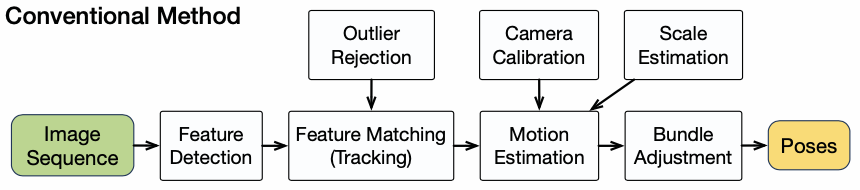
\includegraphics[width=0.75\columnwidth]{figuras/figura1.png}
        %     \caption{Classical pipeline for Visual Odometry.}
        %     \label{fig:1}
        % \end{figure}
        
\end{document}
